Our tomcat server (spring backend) is configured to accept 100 requests at once and queue them in a thread pool consisting of 10 threads per instance, and the container hosting the server is given almost all available RAM from the VM approximately: 2 GM, so we have not needed to scale out the application during the simulation process. However, we were using the vagrant setup on the VM for almost the entire course, and we switched to AKS in the final 2 weeks. Using k8s we have a replica set configured to be replicated 3 times. To manage networking and load balancing, we have configured a routing service that has a static IP address to manage networking, which works as a gateway in front of the pods, see Figure \ref{fig:loadBalancingStable}

\begin{figure}[h]
    \centering
    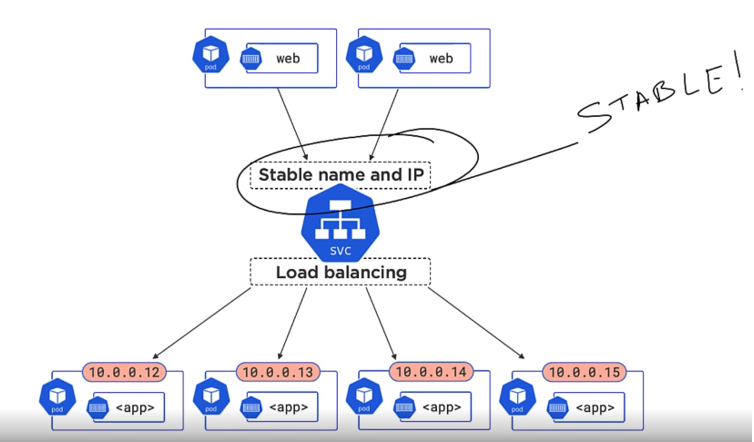
\includegraphics[width = 0.5\textwidth]{loadBalancingStable.png}
    \caption{Load balancing \cite{https://kubernetes.io/KubernetesKubernetes}}
    \label{fig:loadBalancingStable}
\end{figure}

In the current cluster we are performing a rolling update deployment and it works as follows: the scheduler in the master issue a new task to any available node from the node pool, once the task is received and acknowledged by a node, one of the controller watch loop, namely the replica controller, will register the desired state in the deployment manifest and compare it with the current cluster sate to make sure that the cluster is running exactly what is specified in the manifest. The replica set controller will watch, in a loop, the liveliness and liveness probe and the readiness probe for any new created pods and it will align with the networking service or with the load balancer service to start routing some traffic to the new pod, while keeping some of the traffic to the old pods. Once the pod could handle the traffic correctly, the replica controller will kill one of the old pods and replace it with the new one. The same process will continue until all the old pods are killed and replaced with new pods.

